\chapter{Decreasing Power Token}
\label{sec:chamber_721}

% path
% ref of figure to create
% list of accounts
% ref of scenario described
% caption end
% footnote
\NewDocumentCommand{\printPowerFunctionGraphs}{O{p} m m m m o o}{%
\begin{figure*}[#1]
  \begin{tikzpicture}
		\begin{axis}[
		  name=tokens_power,
		  enlarge x limits=false,
		  title=Absolute Power per Account,
		  width=\linewidth,
		  height=\textheight/6,
			xlabel={$t$},
      ylabel={$p_u(t)$},
			ymin=0,
		]
      \foreach \account in {#4}{
        \addplot table {data/#2/absolute/\account.dat};
        \addlegendentryexpanded{Account \uppercase{\account}}
      }
		\end{axis}
		\begin{axis}[
		  at={(tokens_power.below south west)},
		  yshift=-3mm,
		  anchor=above north west,
		  ymin=0,
		  ymax=1,
		  stack plots=y,
		  area style,
		  enlarge x limits=false,
		  title=Relative Power per Account,
		  width=\linewidth,
		  height=\textheight/6,
		  xlabel={$t$},
      ylabel={$q_u(t)$},
		]
		  \foreach \account in {#4}{
        \addplot table {data/#2/relative/\account.dat} \closedcycle;
		  }
		\end{axis}
  \end{tikzpicture}
  \caption{%
  	\label{#3}%
    \cref{#5}\IfValueT{#6}{ #6}%
  }%
  \IfValueT{#7}{%
    \floatfoot{#7}%
  }%
\end{figure*}
}

In this chapter, we propose a new kind of governance token based on the \textsc{erc721} standard: Decreasing Power Token (\textsc{dpt}).
Those tokens are aimed specifically at governance, and we summarize why we think they fulfill this purpose better than existing solutions at the end of the chapter.

\section{\textsc{Dpt} Properties}

\textsc{Dpt}s feature the following properties:

\begin{description}
  \item[Initial Value Rewards Value Provided]
    The initial value of a \textsc{dpt} must be proportional to the value provided to the project during a given time or through a given task.
    A natural moment to award such tokens in the context of open source is at the end of a merge request.
    A scheme to determine the value of the token is proposed in \cref{sec:rewarding_scheme}.
  \item[Non-transferable]
    Once a token is awarded to an account, it can never be transferred to any other%
    \marginNote{%
		  Non-transferability of tokens that implement the \textsc{erc721} standard, is achieved by throwing some exceptions in all the transfer functions required by the standard.
		  This effectively renders any transfer function from the standard unusable.
		}.
  \item[Decreasing Power]
  	The voting power of a token decreases over time.
  	This encodes the fact that you are probably more involved in a project if you contributed recently than if you contributed a long time ago, as projects evolve.
\end{description}

The power of any user $u$ at time $t$ is given by:

\begin{equation}
  \label{eqn:power_of_user_with_decreasing_erc721}
  p_u(t) = \sum_{\tau\in T_u(t)}\tau\mathtt{.power}(t)
\end{equation}

The formula above is very similar to \cref{eqn:power_in_token_based_voting_systems} but the power of a token now additionally depends on the time $t$.

We use the \textsc{erc721} standard, because it is the most minimal standard that is both widely accepted and that provides enough flexibility to store the information required for \textsc{dpt}s.

\section{Decreasing Power Functions}

In this work, we will restrict ourselves, for simplicity, to decreasing functions composed of two additive terms.
One of the terms is decreasing in time, we call it the \emph{variable power}.
For a given token $\tau$, we denote the initial value of the variable power $v_\tau$.
We reserve the variable $a_\tau$ to describe the speed at which the token decreases in any form meaningful for the specific decreasing function used.
We defined the second term of the power of a token to be a constant.
We call it the asymptotic power, as it is the power that remains when the variable power reaches zero, which might happen at $t=\infty$, and denote it $b_\tau$.

The power at mint time is given by $\tau\mathtt{.power}(t_{mint}) = v_\tau + b_\tau$, and the power remaining in a token at $t=\infty$ is $\lim_{t\rightarrow\infty}\tau\mathtt{.power}(t) = b_\tau$.

For any decreasing power function, it is important to analyze how \emph{relative} powers of users $q_u(t)$ evolve, as it is the metric that matters when voting: it determines the impact you have on the DAO.

Asymptotic power is explored in \cref{sec:asymptotic_power}, while some possible decreasing functions are analyzed in \cref{sec:analysis_of_possible_decreasing_functions}.

\section{Asymptotic Power $b$}
\label{sec:asymptotic_power}

The asymptotic power denoted $b_\tau$ is the long-term memory of a token about the value of the contribution provided by its owner.
We examine a few strategies to set the value of $b_\tau$.

\subsection{Absolute Value Asymptotic Power}

\begin{proposition}[Absolute values for $b_\tau$ do not make sense]
  Assume that all tokens have the same absolute value $b$.
  If no new contributions are made for a long time, then all variable power might reach zero value.
  At this point, each person's remaining power will be proportional to the \emph{number} of tokens obtained, not to the value provided.
  We deem this an undesirable outcome.
\end{proposition}

We conclude that it is better to define the asymptotic power as a \emph{percentage} of the total initial power.
But what percentage should we use?

\subsection{Zero Asymptotic Power}
\marginElement{%
  \null\hfill%
  \begin{tikzpicture}[
      every nodes/.style = {
        font=\scriptsize,
      },
    ]
    \graph[
      layered layout,
      grow down,
      branch right,
      edges={
        nodes={
          sloped,
        }
      },
    ] {
      Can variable power reach $0$? ->["yes"] "$b_\tau \ne 0$";
      Can variable power reach $0$? ->["no"] Anything is fine;
    };
  \end{tikzpicture}\hfill\null%
}

Can we set the asymptotic power to zero?
Must we set the asymptotic power to zero?

We need to know whether the \emph{variable} power can reach zero.
In the case of exponential decay, the answer is no, and so token holders will always keep some power from the contributions they made.
In turn, this means that there will always be some power that remains in the DAO.
In this case, we see no restrictions on the asymptotic power.
It can be set to zero, or some non-zero value.

In the case of tokens whose variable power does reach the zero value at some fixed point in time, like linearly decreasing token, if we set the asymptotic power to zero too, then the DAO might end up in a state in which no one has any power over the DAO left.

This voting system is envisioned to be implemented on the blockchain, so \textsc{dpt}s will likely take the form of a smart-contract.
Smart contracts can receive money, which can be useful to incentivize open source projects, which we explore in the subsequent chapters.
What happens when all tokens reach zero value?
Can no one make any decisions for the project anymore?
In such a case the funds would be lost forever, which is undesirable.
Can anyone take control?
But then people might take control of the smart contract only to empty it of its fund, not for the benefit of the project, which is also undesirable.
In any case, we see it more likely that the developers will mint new tokens to themselves (even if they do not produce any new feature), to keep control.
But creating a system that incentivizes its members to hack it is considered undesirable.
So reaching the situation in which no account has any power left is nonsensical, and should be avoided altogether.

\subsection{Optimum Asymptotic Power Value}

What is a reasonable percentage for $b_\tau$?

This is a complex question, which requires analyzing relative power dynamics.
We first take a look at two extreme cases to illustrate what the design space is.

Let's first consider tokens whose power decreases extremely rapidly (though they never actually reach zero).
Assume that the system is so extreme, that if you are the last to obtain a token, you gain dictatorial power.
This implies that power shifts rapidly from one person to the other.
It is a way to give a lot of importance to recency, and no importance to history.
How does a system which gives dictatorial power to a different person every day integrate with our moral philosophy?
Is it a fair system?
Does it provide good guarantees?
To govern an open source system, we deem that such a situation is not desirable.
One reason is that we aim to achieve decentralized power distribution.
No decentralization lowers security guarantees: among the many one-day dictators of the project, one of them will most certainly be an adversarial agent.
Another reason is that power tends to protect and centralize itself.
So, the rewarding scheme used to award new tokens might be abused by the dictator so that they maintain control.

We now consider the opposite case: tokens whose power diminishes infinitely slowly, i.e.\ constant power tokens.
Such tokens are much more common in modern societies, this is how shares of publicly traded companies behave for example%
\marginNote{%
  Why are constant power tokens more common in modern societies?
  One answer is that such tokens are much easier to implement.
  Are they better than \textsc{dpt}s?
  Maybe, but maybe we suffer from familiarity bias when we emit this opinion.
  We recommend that the reader keep an open mind.
}.
As long as no new tokens are created, the relative power of any token remains constant.
Creating new shares dilutes the relative power of previous shareholders.
We do not think that this approach is desirable either for the reasons below.

One reason is that it shrinks the design space for the initiator of a project.
With \textsc{dpt}s it is possible to create tokens whose relative power augments, e.g.\ when the other tokens lose absolute power faster than the current token.

Another reason is power enshrinement.
This system is the opposite of the system described above, which might be proof enough, that stable power tokens enshrine power%
\marginNote{
  To go even further, consider tokens whose value would increase in time.
  In such a situation, being the first to contribute is advantageous because your token will augment during more time than the others, and so there are strong chances that you have the most power.
  Obtaining more power than the first contributors is hard in such a context: power is enshrined.
}.
One can also remark that tokens whose power does not decrease over time do not discount based on the elapsed time since contribution, hence they enshrine power.
We now show more formally, why constant power tokens enshrine power.
When token have constant power, then the total amount of power in a system must be inflationary%
\marginNote{%
  With \textsc{dpt}s, the system might be inflationary (when more power is minted than power decreases), or deflationary (when power decreases faster than it is minted).
}.
Assume that tokens' initial power is drawn from a \emph{stationary} distribution%
\marginNote{
  We deem it desirable that the initial power of tokens comes from a stationary distribution.
  This way, providing the same value in the past, now, or in the future, brings you the same power over the system.
  It prevents strategic behaviors based on timing, and it simplifies the rewarding scheme because it becomes possible to compare with previous rewards to determine the value of a current reward.
}.
When you get a new token, its relative power is obtained by dividing the power of the token by the sum of the power of all the tokens in the system.
If these tokens have decreasing value, then this sum will be smaller, and hence you would obtain more relative power, than in the system with constant power tokens.

This is fundamentally a moral question: for what duration should society concede an advantage as compensation for good deeds.
For example in Switzer\-land, federal counselors, at retirement and provided that they held office for four years at least, benefit from a pension of approximately 225'000CHF per year.
Some are questioning whether it should be abolished.
The state of Geneva abolished in November 2021 the life pension that counselors from the \enquote{Grand Conseil} were entitled to (another effect of the \enquote{Affaire Maudet}).

How important should new contributions be compared to old ones?
We propose that finding a middle ground is the appropriate answer.
Current systems enshrine power too much, making it difficult to bring change, even when many current contributors agree, but a few past contributors disagree.
This makes power transitions too difficult.
For the current system, this means setting $b_\tau$ to percentages that are neither too close to 100\% nor to use percentages too close to 0\%.
Each project is different, so the expectations regarding power entrenchment might vary: some might desire very stable power dynamics, and others might favor a more agile approach.

\section{Analysis of Possible Power Functions}
\label{sec:analysis_of_possible_decreasing_functions}

We now analyze a few decreasing functions to get a feeling of the possible effects of using decreasing power tokens.

\subsection{Scenarios}

For each decreasing function analyzed, we will explore some scenarios, where a scenario is a sequence of mint events.

\begin{scenario}[Identical power at different time steps]
  \label{sce:identical_power_different_time_steps}
  Different accounts receive the same power but at different time steps.

  \begin{center}
    \begin{tabular}{lll}
      \toprule
        \textbf{Time} & \textbf{Receiving Account} & \textbf{Amount of Power}\\
      \midrule
        0 & A & 100\\
        20 & B & 100\\
        40 & C & 100\\
        60 & D & 100\\
        80 & E & 100\\
        100 & F & 100\\
      \bottomrule
    \end{tabular}
  \end{center}
\end{scenario}

\begin{scenario}[Different powers at identical time step]
  \label{sce:different_powers_identical_time_step}
  Tokens of different powers are minted at the same time.

  \begin{center}
    \begin{tabular}{lll}
      \toprule
        \textbf{Time} & \textbf{Receiving Account} & \textbf{Received Amount}\\
      \midrule
        0 & A & 100\\
        0 & B & 80\\
        0 & C & 60\\
        0 & D & 40\\
        0 & E & 20\\
      \bottomrule
    \end{tabular}
  \end{center}
\end{scenario}

\begin{scenario}[Less power later]
  \label{sce:less_power_later}
  An account receives a token of lesser value than another account, but later.

  \begin{center}
    \begin{tabular}{lll}
      \toprule
        \textbf{Time} & \textbf{Receiving Account} & \textbf{Amount of Power}\\
      \midrule
        0 & A & 100\\
        50 & B & 50\\
      \bottomrule
    \end{tabular}
  \end{center}
\end{scenario}

\begin{scenario}[Main contributor]
  \label{sce:main_contributor}
  The main contributor builds half of the features of a project, and various other developers contribute single features.

  \begin{center}
    \begin{tabular}{lll}
      \toprule
        \textbf{Time} & \textbf{Receiving Account} & \textbf{Amount of Power}\\
      \midrule
        0 & A & 100\\
        10 & B & 100\\
        20 & A & 100\\
        30 & C & 100\\
        40 & A & 100\\
        50 & D & 100\\
        60 & A & 100\\
        70 & E & 100\\
      \bottomrule
    \end{tabular}
  \end{center}
\end{scenario}

\subsection{Linear Decay}
\marginElement{%
  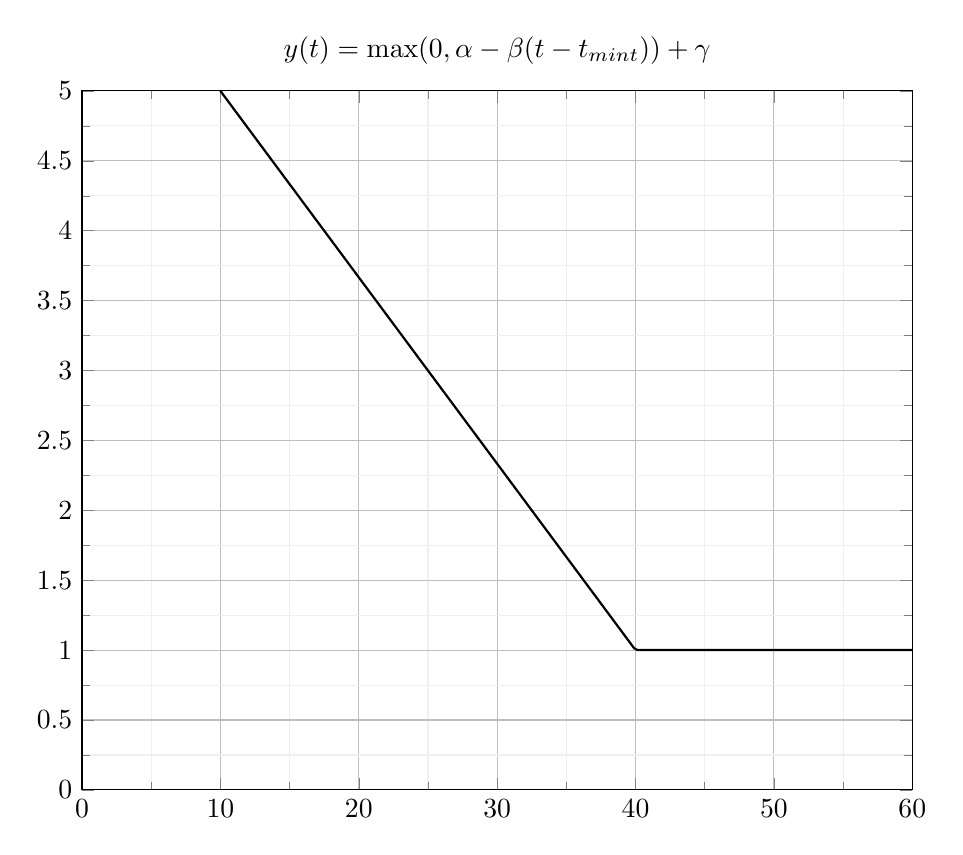
\begin{tikzpicture}
    \begin{axis}[
      xmin = 0, xmax = 60,
      ymin = 0, ymax = 5,
      title = {$y(t) = \max(0, \alpha - \beta (t - t_{mint})) + \gamma$},
      % xtick distance = 2.5,
      % ytick distance = 0.5,
      grid = both,
      minor tick num = 1,
      major grid style = {lightgray},
      minor grid style = {lightgray!25},
      width = \linewidth,
      % height = 0.5\textwidth
    ]
      \addplot[
        domain = 10:60,
        samples = 200,
        thick,
      ] {max(0, -4/30 * (x - 10) + 4) + 1};
    \end{axis}
  \end{tikzpicture}
  \captionof{figure}{\label{fig:linear_decay}Linear Decay}
  \vspace*{\baselineskip}%
  {%
    \small%
    Parameters: $a = \sfrac{4}{30}, t_{mint} = 10, b = 4$ and $c = 1$%
  }
}

Probably the most simple decreasing function to use is the linearly decreasing function.
A visual representation of linear decay is given in \cref{fig:linear_decay}.
The power function of a token $\tau$ is given by:

\begin{equation}
  \label{eqn:linear_decay_power}
  \tau\mathtt{.power}(t) = %
  \begin{cases}
    0 & t < t_{mint}\\
    \max\left(0, v_\tau - a_\tau(t - t_{mint})\right) + b_\tau & \forall t\ge t_{mint}\\
  \end{cases}
\end{equation}

The slope parameter $a_\tau$ of linear decay functions (see \cref{eqn:linear_decay_power}) can be selected in various ways, two of which are intuitive.
One idea is to select the same constant slope for all tokens.
The other is to define an identical duration for all tokens during which they move from their maximal value to their minimal one.

As shown in \cref{sec:asymptotic_power}, it is not possible to use a zero asymptotic power with linearly decreasing tokens.
In all the following examples, we set $b_\tau$ to 50\% of the initial value of the token.

\subsubsection{Constant Slope}

Let's first look at the simplest option, which is to set the same slope for all tokens.
Such a situation is shown in \cref{fig:linear_decay_constant_slope_different_powers_identical_time_step}.

\printPowerFunctionGraphs[ht]%
  {different_powers_identical_time_step/linear_decay_constant_slope}
  {fig:linear_decay_constant_slope_different_powers_identical_time_step}
  {a,...,e}
  {sce:different_powers_identical_time_step}
  [with linear decay with constant slope]

This setup is deemed undesirable because people that obtain tokens with larger values are rewarded doubly: once because their token has large power, and a second time because this power takes a long time to decrease.
If developer rewards are enabled, then the double paying is quite literally happening.

\subsubsection{Constant Time to Asymptotic Power}

\printPowerFunctionGraphs%
  {identical_power_different_time_steps/linear_decay_constant_dt}
  {fig:linear_decay_constant_dt_identical_power_different_time_steps}
  {a,...,e}
  {sce:identical_power_different_time_steps}
  [with linear decay with constant $\Delta t$]

\printPowerFunctionGraphs%
  {different_powers_identical_time_step/linear_decay_constant_dt}
  {fig:linear_decay_constant_dt_different_powers_identical_time_step}
  {a,...,e}
  {sce:different_powers_identical_time_step}
  [with linear decay with constant $\Delta t$]

\printPowerFunctionGraphs%
  {less_power_later/linear_decay_constant_dt}
  {fig:linear_decay_constant_dt_less_power_later}
  {a,...,b}
  {sce:less_power_later}
  [with linear decay with constant $\Delta t$]

\printPowerFunctionGraphs%
  {main_contributor/linear_decay_constant_dt}
  {fig:linear_decay_constant_dt_main_contributor}
  {a,...,e}
  {sce:main_contributor}
  [with linear decay with constant $\Delta t$]

We now consider another approach in which the slope is defined so that the tokens will reach their asymptotic power after a preset time $\Delta t$.
We set this time to 50 time-step in this simulation.
We redefine $a=\sfrac{v_\tau}{\Delta t}$ and remark that this definition satisfies what we are looking for: at $t = t_{mint}$, $\tau\mathtt{.power}(t) = v_\tau + b_\tau$ and at $t \ge t_{mint} + \Delta t$, we have $\tau\mathtt{.power}(t) = b_\tau$.
This setup is illustrated with \crefrange{fig:linear_decay_constant_dt_identical_power_different_time_steps}{fig:linear_decay_constant_dt_main_contributor}.%

In the specific case of tokens with different powers, but minted at the same time, i.e.\ the situation described in \cref{sce:different_powers_identical_time_step}, note that relative powers between these tokens remain identical (\cref{fig:linear_decay_constant_dt_different_powers_identical_time_step}).
This does not hold when the token are minted at different time steps however (see \cref{fig:linear_decay_constant_dt_identical_power_different_time_steps}).

We do not see obvious problems with the results of linearly decreasing power tokens with constant time to asymptotic power.
Some real-life experimentations are required.

\subsection{Exponentially Decreasing Function}

\leavevmode\marginElement{%
  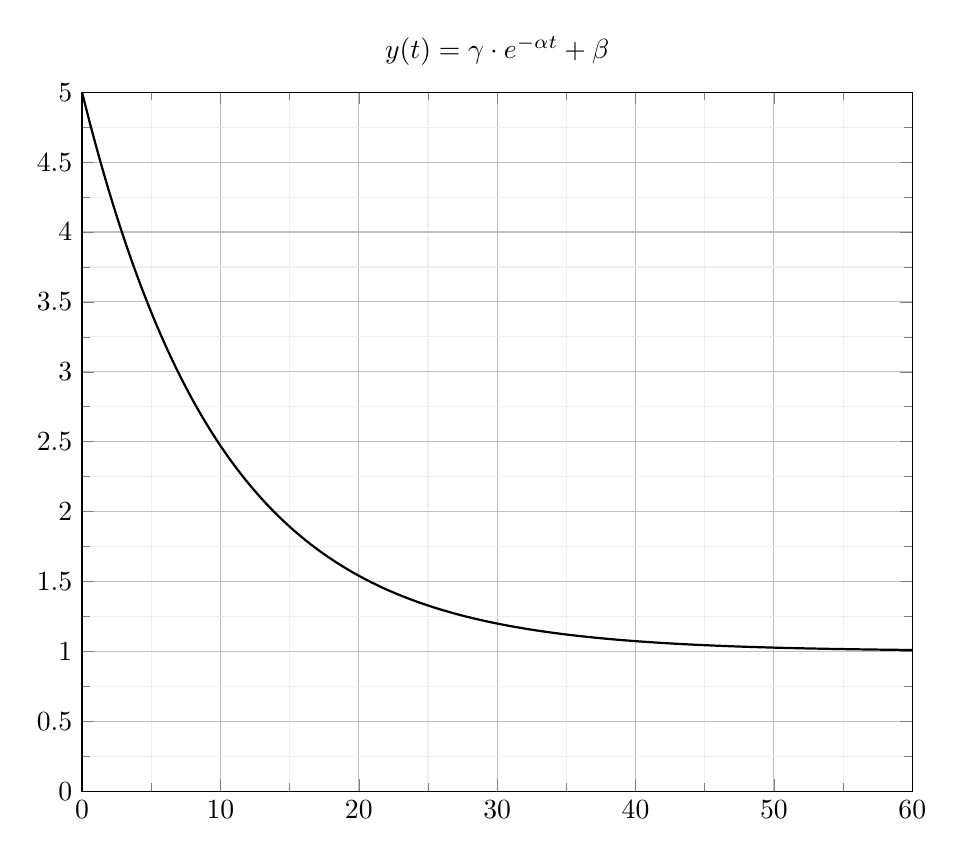
\begin{tikzpicture}
    \begin{axis}[
      xmin = 0, xmax = 60,
      ymin = 0, ymax = 5,
		  title = {$y(t) = \gamma \cdot e^{-\alpha t} + \beta$},
      % xtick distance = 2.5,
      % ytick distance = 0.5,
      grid = both,
      minor tick num = 1,
      major grid style = {lightgray},
      minor grid style = {lightgray!25},
      width = \linewidth,
      % height = 0.5\textwidth
    ]
      \addplot[
        domain = 0:60,
        samples = 200,
        smooth,
        thick,
      ] {4 * exp(-x/10) + 1};
    \end{axis}
  \end{tikzpicture}
  \captionof{figure}{\label{fig:exponential_decay}Exponential decay}
  \vspace*{\baselineskip}%
  {%
    \small%
    Parameters: $\gamma = 4$, $\alpha = \sfrac{1}{10}$ and $\beta = 1$%
  }
}%
Exponential functions come up rather frequently in nature, so it might be a worthwhile function to explore.
A visual representation of exponential decay is given in \cref{fig:exponential_decay}.
Below is the mathematical formula of the power of an exponential decay \textsc{erc721} token $\tau$:

\begin{equation}
  \label{eqn:power_of_exponential_decay_erc721}
  \tau\mathtt{.power}(t) = v_\tau \cdot e^{-a'_\tau (t - t_{mint})} + b_\tau
\end{equation}

A disadvantage of exponential decay functions is that they are harder to understand for humans, which makes the system more complex.

We define $a_\tau$ as the half-life of the function, i.e. the time after which the value of the function is halved.
For a half-life of $5$ time units, the coefficient $a'_\tau$ in the exponential must satisfy $a'_\tau = \sfrac{\ln(2)}{a_\tau} = \sfrac{\ln(2)}{5}$.

\subsubsection{Exponential Decay with Zero Asymptotic Power}

\printPowerFunctionGraphs%
  {identical_power_different_time_steps/exponential_decay_30_0}
  {fig:exponential_decay_30_0_identical_power_different_time_steps}
  {a,...,e}
  {sce:identical_power_different_time_steps}
  [with exponential decay with $a_\tau=30$ and $b_\tau=0\%$]

\printPowerFunctionGraphs%
  {different_powers_identical_time_step/exponential_decay_30_0}
  {fig:exponential_decay_30_0_different_powers_identical_time_step}
  {a,...,e}
  {sce:different_powers_identical_time_step}
  [with exponential decay with $a_\tau=30$ and $b_\tau=0\%$]

\printPowerFunctionGraphs%
  {less_power_later/exponential_decay_30_0}
  {fig:exponential_decay_30_0_less_power_later}
  {a,...,b}
  {sce:less_power_later}
  [with exponential decay with $a_\tau=30$ and $b_\tau=0\%$]

\printPowerFunctionGraphs%
  {main_contributor/exponential_decay_30_0}
  {fig:exponential_decay_30_0_main_contributor}
  {a,...,e}
  {sce:main_contributor}
  [with exponential decay with $a_\tau=30$ and $b_\tau=0\%$]

The situation with exponential decay and no asymptotic power is described in \crefrange{fig:exponential_decay_30_0_identical_power_different_time_steps}{fig:exponential_decay_30_0_main_contributor}.%

Exponential functions with zero asymptotic power and identical half-lives have identical relative decreases over the same period.
So given that no mint event occur, i.e.\  $T(t_0) = T(t_0 + \Delta t)$, the relative power $q_u(t)$ of every user $u$ will remain identical between $t_0$ and $t_0 + \Delta t$.
This effect can be witnessed in \cref{fig:exponential_decay_30_0_different_powers_identical_time_step}.
Here is a quick proof:

\begin{equation*}
  \begin{aligned}
    q_u(t_0 + \Delta t) &\overset{\ref{eqn:relative_power}}{=} \frac{p_u(t_0 + \Delta t)}{\sum_{v\in U}p_v(t_0 + \Delta t)}\\
    &\overset{\ref{eqn:power_of_user_with_decreasing_erc721}}{=} \frac{\sum_{\tau\in T_u(t_0 + \Delta t)}\tau\mathtt{.power}(t_0 + \Delta t)}{\sum_{\tau\in T(t_0 + \Delta t)}\tau\mathtt{.power}(t_0 + \Delta t)}\\
    &\overset{\ref{eqn:power_of_exponential_decay_erc721}}{=} \frac{\sum_{\tau\in T_u(t_0+\Delta t)}p_\tau\cdot e^{-a'_\tau (t_0 + \Delta t)}}{\sum_{\tau\in T(t_0+\Delta t)}p_\tau\cdot e^{-a'_\tau (t_0 + \Delta t)}}\\
    &= \frac{\sum_{\tau\in T_u(t_0+\Delta t)}p_\tau\cdot e^{-a'_\tau t_0}\cdot e^{-a'_\tau\Delta t}}{\sum_{\tau\in T(t_0+\Delta t)}p_\tau\cdot e^{-a'_\tau t_0}\cdot e^{-a'_\tau\Delta t}}\\
    &= \frac{\sum_{\tau\in T_u(t_0)}p_\tau\cdot e^{-a'_\tau t_0}}{\sum_{\tau\in T(t_0)}p_\tau\cdot e^{-a'_\tau t_0}}\\
    &= \frac{p_u(t_0)}{\sum_{v\in U}p_v(t_0)}\\
    &= q_u(t_0)
  \end{aligned}
\end{equation*}

This means that it is possible to replicate the semantics of constant value token, i.e.\ relative power that remains identical as long as there are no mints, yet to provide some advantage based on the recency of the contribution.
The size of the advantage is fixed by $a_\tau$.
\Cref{fig:exponential_decay_30_0_identical_power_different_time_steps_comparison} which depicts the relative power of each users at $t=100$ and $t=200$ highlights this.
On the one hand, the users that made contributions more recently have more power than those that contributed longer ago.
On the other hand, the relative power relationships remain constant over time as long as there are no new mints, and indeed the two pies are identical.

\begin{figure*}[ht!]
  \centering
  \begin{tikzpicture}
    \path[%
      /DiagCirc/.cd,
      value list={6.5/A, 10.3/B, 16.3/C, 25.8/D, 41.1/E},
      diagram,
    ];
    \node[
      anchor=south,
    ] at (0, 3.2cm) {$t=100$};
	\end{tikzpicture}
  \hspace*{10mm}%
  \begin{tikzpicture}
    \path[
      /DiagCirc/.cd,
      value list={6.5/A, 10.3/B, 16.3/C, 25.8/D, 41.1/E},
      diagram,
    ];
    \node[
      anchor=south,
    ] at (0, 3.2cm) {$t=200$};
  \end{tikzpicture}
  \caption{%
  	\label{fig:exponential_decay_30_0_identical_power_different_time_steps_comparison}%
    Relative power at $t=100$ and $t=200$ in \cref{sce:different_powers_identical_time_step} with exponential decay and no asymptotic power.
  }
  \floatfoot{%
    All the users in the above pies contributed the same value but at different time steps.
    The recency advantage is rather clear: user F has more relative power than user E, which itself has more than user D, etc.
    Using exponential decay and setting asymptotic power to $0\%$ further implies that relative power relationships remain identical over time, as long as there are no mint events.
    This is showcase above in that the relative power relationships are identical at $t=100$ and $t=200$.
  }
\end{figure*}

\subsubsection{Exponential Decay with Non-Zero Asymptotic Power}

\printPowerFunctionGraphs%
  {identical_power_different_time_steps/exponential_decay_30_50}
  {fig:exponential_decay_30_50_identical_power_different_time_steps}
  {a,...,e}
  {sce:identical_power_different_time_steps}
  [with exponential decay with $a_\tau=30$ and $b_\tau=50\%$]

\printPowerFunctionGraphs%
  {different_powers_identical_time_step/exponential_decay_30_50}
  {fig:exponential_decay_30_50_different_powers_identical_time_step}
  {a,...,e}
  {sce:different_powers_identical_time_step}
  [with exponential decay with $a_\tau=30$ and $b_\tau=50\%$]

\printPowerFunctionGraphs%
  {less_power_later/exponential_decay_30_50}
  {fig:exponential_decay_30_50_less_power_later}
  {a,...,b}
  {sce:less_power_later}
  [with exponential decay with $a_\tau=30$ and $b_\tau=50\%$]

\printPowerFunctionGraphs%
  {main_contributor/exponential_decay_30_50}
  {fig:exponential_decay_30_50_main_contributor}
  {a,...,e}
  {sce:main_contributor}
  [with exponential decay with $a_\tau=30$ and $b_\tau=50\%$]

The situation with exponential decay and asymptotic power set to 50\% of the initial value of the token is described in \crefrange{fig:exponential_decay_30_50_identical_power_different_time_steps}{fig:exponential_decay_30_50_main_contributor}.%

By setting the asymptotic power to a higher percentage of the total power granted, for example, $b=50\%$, the system gives more weight to historical events, than the case in which the asymptotic power is set to zero.

\Cref{fig:exponential_decay_30_50_identical_power_different_time_steps_comparison} shows that the system first goes through some transitory phase during which more recent contributions are advantaged.
Then, as the variable power of all tokens decreases, the system returns to a situation in which the total power owned by each user is proportional to the value contributed in the entire history of the project.
In a sense, the project gives an advantage to recent contributions if there are some, and otherwise returns to distributing power according to the history of value provided.

\begin{figure*}[ht!]
  \centering
  \begin{tikzpicture}
    \path[%
      /DiagCirc/.cd,
      value list={16.8/A, 17.7/B, 19.1/C, 21.4/D, 25.0/E},
      diagram,
    ];
    \node[
      anchor=south,
    ] at (0, 3.2cm) {$t=100$};
	\end{tikzpicture}
  \hspace*{10mm}%
  \begin{tikzpicture}
    \path[
      /DiagCirc/.cd,
      value list={19.6/A, 19.7/B, 19.9/C, 20.2/D, 20.6/E},
      diagram,
    ];
    \node[
      anchor=south,
    ] at (0, 3.2cm) {$t=200$};
  \end{tikzpicture}
  \caption{%
  	\label{fig:exponential_decay_30_50_identical_power_different_time_steps_comparison}%
    Relative power at $t=100$ and $t=200$ in \cref{sce:different_powers_identical_time_step} with exponential decay and asymptotic power set to 50\% of the initial power of the token.
  }
  \floatfoot{%
    In the first pie, the variable power of the first minted token has largely decreased, but the most recent tokens do not yet have lost this value.
    Thus the most recent contributions are rewarded with more relative power.
    But if no new contributions are made, then the variable power of all tokens diminishes, and the power distribution converges to giving the same relative power to everyone as everyone contributed the same value to the project though at different time steps in this scenario.
  }
\end{figure*}

\section{Are \textsc{dpt} Good for Governance Purposes?}
\label{sec:dpt_philosophical_analysis}

What are the benefits of using \textsc{dpt}s over constant value tokens?
Are there limitations?
We explore these questions in this section.

\subsection{Timing Strategies}

We first consider whether there might exist strategic behaviors that exploit time.
Might actors have incentives to wait before contributing, or is it always better to contribute as soon as possible?
We consider that any project should aim for agents to contribute as soon as possible because it increases the speed of development.

In the following discussion, we define $v_u(t, q_u(t))$ as the private valuation that user $u$ has for owning $q_u(t)$ relative power at time $t$, and $v_u$ as the total value that user $u$ gets over time.
The variable $v_u$ could be called user $u$'s \emph{interest}, as it is the total private value that user $u$ obtains from the power they own over time:

\begin{align*}
  v_u &= \sum_{t=0}^\infty v_u(t, q_u(t))\\
  &= \sum_{t=0}^\infty v_u\left(t, \frac{\sum_{\tau\in T_u(t)}\tau\mathtt{.power}(t)}{\sum_{\tau\in T(t)}\tau\mathtt{.power}(t)}\right)\\
\end{align*}

We keep $q_u(t)$ a parameter of $v_u$, instead of defining, for example, the value per unit of relative power at time $t$ as a constant, because the marginal utility of the relative power might not be constant%
\marginNote{%
  In the case of money, for example, it is generally accepted that for most humans money had a diminishing utility, i.e.\ the more money you have, the less you care about earning an additional dollar.%
}.

Let's first consider the case in which asymptotic power is zero, $b = 0\%$, and assume you know that no one other than you will contribute to the project: $T_{-u}(t_1) = T_{-u}(t)\forall t\ge t_1$, where $T_{-u}$ designates the set of the set of tokens owned by each user, except that of user $u$.
This case, although specific, is interesting, because there might be reason enough to delay a contribution.
In this context, if you contribute later, you get more relative power because the power of the others diminishes when you wait.
This is illustrated in \cref{fig:exponential_decay_30_0_identical_power_different_time_steps}; account E, by contributing later, gets a large share of relative power.
If they had waited for more, they would have gotten even more relative power.
And as we assume that we have oracle knowledge that no other contributions will be made, depending on the decreasing function used by the token, we might keep this large relative power share.
But the period during which you do not contribute must also be considered: having no power during this period has a cost, as illustrated by the equation above which sums over all time steps.
So the situation is not clear and depends on your private valuation for having some power early versus having more power later, and on the decreasing function used.

In projects with no asymptotic power, but in which contributions of similar value are made at regular intervals, contributing early or late does not make a difference.
Through our assumptions, and given that the function used for the tokens decays fast enough, we can also assume that the total amount of absolute power in the system will be approximately constant over time.
Hence, there is no clear incentive to make your contribution early or late, as it will grant you the same amount of relative power over time, irrelevant of the specific moment you contribute.

In projects with non-zero asymptotic power, contributing early in the history of the project is better because of inflation.
In \cref{fig:exponential_decay_30_0_identical_power_different_time_steps} for example, account A, by contributing early, obtains a lot more relative power over the history of the project, than account E.
This means that during the early days of the project, so days 0 to 60 approximately, account A can influence the project a lot.

Even with decreasing power tokens, there is no clear case for the existence of strategic behaviors exploiting timing.
Even if there might exist specific circumstances under which users might have an incentive to wait before contributing, the effect of inflation, the loss of relative power during the period in which you withhold your contribution, and the effect that contributions made after yours will have on your power are all incentives to contribute early and as soon as possible.
Having some amount of asymptotic power, in other words, a little bit of inflation seems to improve guarantees.

Another kind of timing strategy is to vote later than one would have normally done, to have more relative power at the moment of voting.
With \textsc{dpt}s this is possible, as there are situations in which waiting and doing nothing will grant you more relative power.
However, provided that the voting periods are short, and that the time intervals across which tokens decrease in power are long, the effects of such strategies are negligible.

\subsection{Speculation on the Value of Governance Token}

The value of governance power is often hard to estimate, yet, because \textsc{dpt} tokens are non-transferable, there can be no market for them, and they can have no value.
Indeed, if you cannot obtain something, then it makes no sense to talk about the value it would bring you.
This disincentivizes people that would contribute to speculate on the future value of the governance token.
It has indeed been an issue for blockchain-based projects, that people have \enquote{participated} (often in very limited ways), only to obtain some token they hoped the value of would increase over time.
This was the airdrop frenzy.
But these people are seldomly interested in the project or aligned with its ideas.
This is also one of the potential core reasons for the success of the open source: as there is so little monetary incentive to participate, people that do participate often do it because they truly align with the project.

There is a way to hack the non-transferability of the token, namely to use a smart contract as a token holder instead of an Externally Owned Account (EOA).
The smart contract might then sell its voting power to the highest bidder.
The smart contract awarding the tokens could assert that the tokens are only minted to EOA.
This can be counter-acted by selling your voting power using regular off-chain mechanisms.
Setting up such a system implies a lot of friction, so we assume that it is not too likely.

\subsection{Sybil Resistance}

Token-based voting, with fixed-value tokens, is sybil resistant.
We claim that \textsc{dpt}s are also sybil resistant.
An intuitive way to convince yourself of this is that the decreasing functions only use the value of the tokens and time as parameters, and are never related to the account that owns the token.
In a sense, the proposed tokens are self-contained, like \textsc{erc20}s.
We prove this mathematically hereafter.
We define two scenarios, in the first scenario user $u$ has only one account that contains all the tokens.
In the second scenario, user $u$ splits their tokens across multiple account that we name $a_0$, $a_1$, ... $a_k$.

\begin{align*}
  \sum_{a_i} q_{a_i}(t) &= \sum_{a_i}\frac{\sum_{\tau\in T_{a_i}(t)}\tau\mathtt{.power}(t)}{\sum_{\tau\in T(t)}\tau\mathtt{.power}(t)}\\
  &= \frac{\sum_{a_i}\sum_{\tau\in T_{a_i}(t)}\tau\mathtt{.power}(t)}{\sum_{\tau\in T(t)}\tau\mathtt{.power}(t)}\\
  &\overset{(1)}{=} \frac{\sum_{\tau\in T_u(t)}\tau\mathtt{.power}(t)}{\sum_{\tau\in T(t)}\tau\mathtt{.power}(t)}\\
  &= q_u(t)\\
\end{align*}

Where equality (1) holds because the absolute power of any token only depends on values relative to the token itself, but is completely independent of the account that holds it.

Defining the decrease of token proportionally to the total amount of power that a person holds enables per person intrinsic progressive decentralization (defined in \cref{sec:governance_system_chamber_721_intrinsic_power_decentralization}) which we deem a desirable goal.
But without some proof of personhood system (see \cref{sec:sybil_resistance}), i.e.\ if we were to use accounts as proxies for persons, this opens the door to sybil attacks.

\subsection{Making Informed Decisions}

One advantage of decreasing power tokens is that they incentivize renewed contributions.
As there is less power entrenchment, either you keep contributing, or you will lose relative power.
In other words, if you have power over the project, then it must be the case that you are actively involved with the project.
This is positive from the perspective of making informed decisions.

\subsection{Incentive to Keep Contributing}

For people that want to keep some control over the project, or for those that want to keep obtaining rewards when developer rewards are enabled, they have an incentive to contribute value actively to the project, otherwise, they will be outshined by newer contributors who will get the larger part of power and rewards.

\subsection{Extrinsic Power Decentralization}

\textsc{Dpt}s, because they entrench power less, are newcomers friendly.
As a newcomer, you have more guarantees that you can rapidly have some impact on the project, than when there is a lot of power entrenchment%
\marginNote{%
  This applies to many systems.
  Compare, for example, your chances, as a newcomer, of impacting a royalty-based system, and a democratic system.
}.
Having low entry barriers drives extrinsic power decentralization.
In this regard, \textsc{dpt}s have better properties than explicit role systems like GitHub (full power entrenchment), and constant value token systems (more power entrenchment than \textsc{dpt}s).

\subsection{Intrinsic Power Decentralization}
\label{sec:governance_system_chamber_721_intrinsic_power_decentralization}

While GitDao might feature extrinsic decentralization, we would prefer that it features intrinsic decentralization as it is a more robust way to decentralize power.
The proposed \textsc{dpt} are akin to a meritocracy, this means that they do not intrinsically distribute power across humans.
Can we build a system that decentralizes power in a per-person fashion instead of per merit?

We postulate that it is impossible to achieve per-person intrinsic progressive decentralization if we lack proof of personhood.
Intuitively, a system cannot use a discriminating property, if it does not know about it.

\subsection{Large and Small Contributions}

The specific decreasing function used might create different incentives when it comes to the size of the contributions.
In the open source, it is generally speaking a good policy to keep contributions small and to create different merge requests for different contributions.
The reason is that it makes reviewing the merge request much more manageable: many small tasks are easier to do than one big task.

Adding many small linearly decreasing tokens with constant time to asymptotic power is identical to creating one large linearly decreasing token with the same time to asymptotic power.
So in the case of linearly decreasing tokens with constant time to asymptotic power, many small contributions or one big contribution grant the same power.

This is not true of linearly decreasing tokens with a constant slope.
In such a case, it is better to create one large token, than to have multiple smaller ones totaling the same initial power, because the larger token will keep some power for a longer time.

When it comes to exponentially decreasing tokens, creating many small tokens or one large token yields identical results.

It might be desirable to look for decreasing functions that incentivize smaller contributions, i.e.\ functions such that the addition of many smaller tokens yields more relative power than one big token, so super-additive tokens.

\subsection{Trust}

We assume that the tokens have a value that is proportional to the value contributed to the project.
Further, those tokens are not transferable.
This means that if you own some tokens, then you must have provided some value to the project.
Assuming that providing said value required some work (which seems a reasonable assumption: no free lunch), then owning a token is proof that you worked for the project.
As such it can be considered that owning a token acts like a trust gate: if you own a token, then you are probably aligned with the project and can be trusted to do what you feel is right for the project.
The trust comes from the fact that if you want to harm the project, then you would probably not benefit the project in the first place by contributing to it.

Large actors like states might have enough resources to finance developers to contribute to a project to gain enough power over the project to be able to harm it in the future.
But performing such an attack is expensive if the power is decentralized enough, the power over the project needs to be maintained, and if an adversarial agent takes over, it is still possible for the community to fork (though forking is not as easy to do when the project has a bank account).

